\documentclass[tikz,border=5pt]{standalone}
\usepackage{luatexja}
\usepackage[hiragino-pron]{luatexja-preset}
\usepackage{amsmath,amssymb}
\usepackage{pgfplots}
\pgfplotsset{compat=1.18}
\usetikzlibrary{arrows.meta,calc,decorations.markings,patterns,positioning}

% Common styles
\tikzset{
  axis/.style={-{Stealth[length=6pt]}, thick},
  curve/.style={thick, red},
  dashed curve/.style={thick, dashed, blue},
  dot/.style={circle, fill, inner sep=1.5pt},
  open dot/.style={circle, draw, fill=white, inner sep=1.5pt},
}

\begin{document}
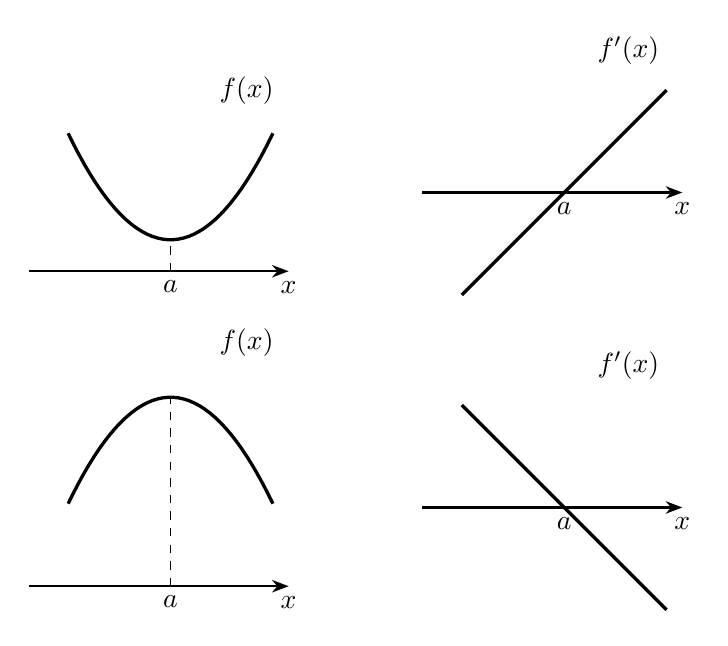
\begin{tikzpicture}

  % Top-left: smooth minimum f(x)
  \begin{scope}
    \draw[axis] (-0.3,0) -- (3,0) node[below] {$x$};
    \node[above right] at (2,2) {$f(x)$};
    \draw[very thick, domain=0.2:2.8, samples=40] plot (\x, {0.8*(\x-1.5)^2+0.4});
    \draw[dashed, semithick] (1.5,0) -- (1.5,0.4);
    \node[below] at (1.5,0) {$a$};
  \end{scope}

  % Top-right: f'(x) for minimum — crosses zero upward at x=a
  \begin{scope}[xshift=5cm, yshift=1cm]
    \draw[axis] (-0.3,0) -- (3,0) node[below] {$x$};
    \node[above right] at (1.8,1.5) {$f'(x)$};
    \draw[very thick, domain=0.2:2.8, samples=30] plot (\x, {1.0*(\x-1.5)});
    \node[below] at (1.5,0) {$a$};
  \end{scope}

  % Bottom-left: smooth maximum f(x)
  \begin{scope}[yshift=-4cm]
    \draw[axis] (-0.3,0) -- (3,0) node[below] {$x$};
    \node[above right] at (2,2.8) {$f(x)$};
    \draw[very thick, domain=0.2:2.8, samples=40] plot (\x, {-0.8*(\x-1.5)^2+2.4});
    \draw[dashed, semithick] (1.5,0) -- (1.5,2.4);
    \node[below] at (1.5,0) {$a$};
  \end{scope}

  % Bottom-right: f'(x) for maximum — crosses zero downward at x=a
  \begin{scope}[xshift=5cm, yshift=-3cm]
    \draw[axis] (-0.3,0) -- (3,0) node[below] {$x$};
    \node[above right] at (1.8,1.5) {$f'(x)$};
    \draw[very thick, domain=0.2:2.8, samples=30] plot (\x, {-1.0*(\x-1.5)});
    \node[below] at (1.5,0) {$a$};
  \end{scope}

\end{tikzpicture}
\end{document}
